\documentclass{article}\usepackage[]{graphicx}\usepackage[]{color}
%% maxwidth is the original width if it is less than linewidth
%% otherwise use linewidth (to make sure the graphics do not exceed the margin)
\makeatletter
\def\maxwidth{ %
  \ifdim\Gin@nat@width>\linewidth
    \linewidth
  \else
    \Gin@nat@width
  \fi
}
\makeatother

\definecolor{fgcolor}{rgb}{0.345, 0.345, 0.345}
\newcommand{\hlnum}[1]{\textcolor[rgb]{0.686,0.059,0.569}{#1}}%
\newcommand{\hlstr}[1]{\textcolor[rgb]{0.192,0.494,0.8}{#1}}%
\newcommand{\hlcom}[1]{\textcolor[rgb]{0.678,0.584,0.686}{\textit{#1}}}%
\newcommand{\hlopt}[1]{\textcolor[rgb]{0,0,0}{#1}}%
\newcommand{\hlstd}[1]{\textcolor[rgb]{0.345,0.345,0.345}{#1}}%
\newcommand{\hlkwa}[1]{\textcolor[rgb]{0.161,0.373,0.58}{\textbf{#1}}}%
\newcommand{\hlkwb}[1]{\textcolor[rgb]{0.69,0.353,0.396}{#1}}%
\newcommand{\hlkwc}[1]{\textcolor[rgb]{0.333,0.667,0.333}{#1}}%
\newcommand{\hlkwd}[1]{\textcolor[rgb]{0.737,0.353,0.396}{\textbf{#1}}}%

\usepackage{framed}
\makeatletter
\newenvironment{kframe}{%
 \def\at@end@of@kframe{}%
 \ifinner\ifhmode%
  \def\at@end@of@kframe{\end{minipage}}%
  \begin{minipage}{\columnwidth}%
 \fi\fi%
 \def\FrameCommand##1{\hskip\@totalleftmargin \hskip-\fboxsep
 \colorbox{shadecolor}{##1}\hskip-\fboxsep
     % There is no \\@totalrightmargin, so:
     \hskip-\linewidth \hskip-\@totalleftmargin \hskip\columnwidth}%
 \MakeFramed {\advance\hsize-\width
   \@totalleftmargin\z@ \linewidth\hsize
   \@setminipage}}%
 {\par\unskip\endMakeFramed%
 \at@end@of@kframe}
\makeatother

\definecolor{shadecolor}{rgb}{.97, .97, .97}
\definecolor{messagecolor}{rgb}{0, 0, 0}
\definecolor{warningcolor}{rgb}{1, 0, 1}
\definecolor{errorcolor}{rgb}{1, 0, 0}
\newenvironment{knitrout}{}{} % an empty environment to be redefined in TeX

\usepackage{alltt}

\title{Draft Outline -- SAS Report}
\author{2016 EA30 Students}
\IfFileExists{upquote.sty}{\usepackage{upquote}}{}
\begin{document}
\SweaveOpts{concordance=TRUE}

\maketitle

\newpage
\tableofcontents
\newpage

\section{Introduction}

\subsection{Problem Statement}
<<<<<<< HEAD
This report aims to determine whether the Biochemical Oxygen Demand (BOD) and water flow velocity are relevant to future conservation research for the endangered Santa Ana sucker \emph{C. santaanae}. The experiment seeks to gather information on the water quality of a section of the Santa Ana River and use this data to help answer the questions: \emph{Are the biochemical oxygen demand (BOD) levels healthy for sucker}, \emph{do differing levels affect the  abundance of individuals in certain sections of the river}, \emph{Are the flow rates in certain sections of the river optimum for sucker populations}, and \emph{do high- or low-flow events affect the number of individuals in the stream?} Because the river is regulated by a water treatment facility, we believe that BOD levels will be very low, increasing with distance from the facility. Because of this, we also expect high dissolved oxygen (DO) content and a high sucker presence. We additionally hypothesize that larger populations of the sucker will concentrate in low-flow areas that are nearby high-flow sections. Through this experiment, we aim to inform Santa Ana sucker conservation efforts and hope to inform action by the nearby water treatment facility. 
=======
This report aims to determine whether the Biochemical Oxygen Demand (BOD) and water flow velocity are relevant to future conservation research for the endangered Santa Ana sucker \emph{C. santaanae}. The experiment seeks to gather information on the water quality of a section of the Santa Ana River and use this data to help answer the questions: \emph{Are the biochemical oxygen demand (BOD) levels healthy for sucker}; \emph{do differing levels affect the  abundance of individuals in certain sections of the river}; \emph{are the flow rates in certain sections of the river optimum for sucker populations}; and \emph{do high- or low-flow events affect the number of individuals in the stream?} Because the river is regulated by a water treatment facility, we believe that BOD levels will be very low, increasing with distance from the facility. We also expect high dissolved oxygen (DO) content and a high sucker presence. Through this experiment, we aim to inform Santa Ana sucker conservation efforts and hope to inform action by the nearby water treatment facility. 
>>>>>>> 261e133571febec3c181725cb6cc9cbdb781d589


\subsection{Background (Literature Review)}
In general, fish have been known to be at risk of suffocation when exposed to dissolved oxygen (D.O.) levels below 2 mg/L for only short periods of time[2]. A 2012 U.S. Fish and Wildlife Service report on the recovery of the endangered fish noted that specific tolerances to dissolved oxygen have not been determined for  Santa Ana Sucker[1]. The 2012 FWS report also notes that constant water flows are important to the availability of coarse substrate which the Sucker needs to spawn offspring and hide from predators. According to Evans et al. (2005), temporary reduction of flows can significantly reduce the amount of habitat for suckers.[3] Just last month, the Center for Biological Diversity reported that ``by halting water releases critical to maintaining surface flows of the Santa Ana River, the Rapid Infiltration and Extraction (RIX) treatment plant is stranding and killing threatened fish.'' [4]

\subsection{Objectives}
We measured BOD levels and water flow velocity in different areas of the Santa Ana River and correlated those measurements with camera observations of Sucker abundance in both sample locations.
\begin{quote}
Our null hypotheses are H0: Water flow velocity and/or BOD levels do not significantly correlate with prevalence of the Santa Ana Sucker.
\end{quote}
\begin{quote}
Our alternative hypotheses are H1: Water flow velocity and/or BOD levels significantly correlate with prevalence of the Santa Ana Sucker.
\end{quote}
If we can reject one or both of our null hypotheses, we can conclude that the study of Biological Oxygen Demand (BOD) and water flow velocity are relevant to future conservation research for the endangered Santa Ana sucker \emph{C. santaanae}.

\section{Methods}

\subsection{Site Descrition}

We evaluated the Santa Ana River between... near Colton, California (Figure \ref{SAR_Image}). 

\begin{figure}
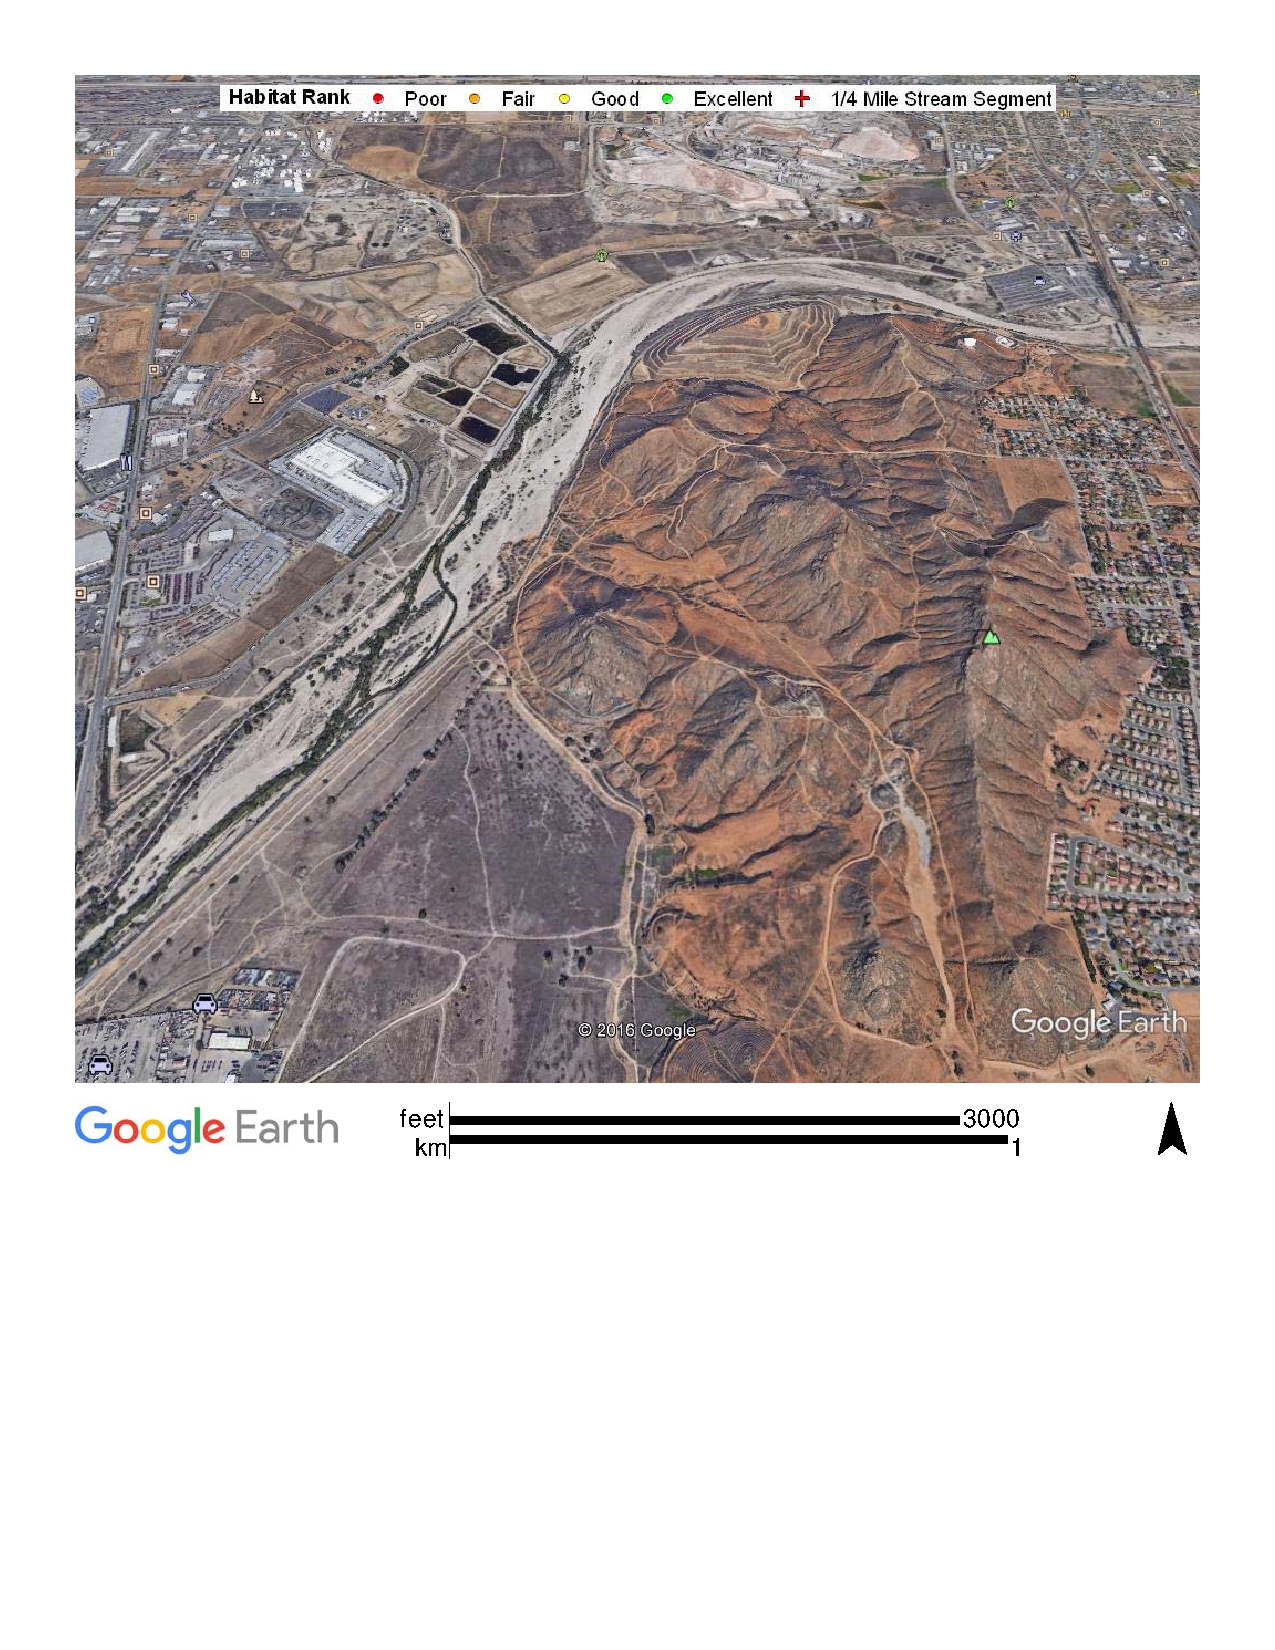
\includegraphics[width=1.00\textwidth]{Figures/SantaAna_SatelliteImage}
\caption{Google Earth --Example of a map. What's wrong with this image?}
\label{SAR_Image}
\end{figure}

\subsection{Field Methods}
\subsubsection*{5-Day Biochemical Oxygen Demand Test (BOD5)}
Approximately 1L of source river water was collected at each of two sites, one upstream location closer to the wastewater discharge facility, and one downstream location (fig. 1), which was transported to the laboratory for analysis within four hours.

\subsubsection*{Water Velocity Collection}
At each of the corresponding water sample collection sites, water velocity was also measured using a SonTek FlowTracker Handheld Advanced probe, which emits sonar waves at a certain depth in the water column, and based on the feedback (20 pings) gives a velocity reading. Ideally, multiple readings would be taken at each site, after the probe is placed on a flat section of the riverbed where water appears to be flowing in the same direction. 

\subsection{Laboratory Methods}
\subsubsection*{BOD5}
Ideally within the same day of collection, water samples are analyzed for initial dissolved oxygen content and prepared for 5-day incubation.  
\begin{itemize}
  \item Three different dilutions were used for each of two sites, with source water volumes of 25, 50, and 100 mL. 
  \item A seed suspension was prepared using PolySeed Seed Innoculum, and 4 mL of the solution was added to each 300 mL sample bottle. This solution was also used to create four seed blanks with seed volumes 15, 20, 25, and 30 mL.
  \item Nitrification inhibitor was created by dissolving 2.0 g allylthiourea (ATU, C4H8N2S) in 1 L distilled water. 0.3 mL of the ATU solution was added to each source water sample, as well as to all seeded samples. 
  \item A glucose-glutamic acid (GGA) solution was prepared by dissolving 150 mg each of dry glucose and glutamic acid in 1 L of distilled water, and was added to each of the four seed blanks, as well as the six source water samples. Three GGA blanks were also created with 6 mL of GGA solution in incubation bottles. 
  \item Dilution water was created using 1 mL each phosphate buffer (8.5 g KH2PO4, 21.75 g K2HPO4, 33.4 g Na2HPO*7H2O, and 1.7 g NH4Cl dissolved in 1 L distilled water), Magnesium sulfate solution (4.5 g MgSO4*7H2O dissolved in 200 mL distilled water), Calcium chloride solution (5.5 g CaCl2 dissolved in 200 mL distilled water), and Ferric chloride solution (0.05 g FeCl3*6H2O dissolved in 200 mL distilled water), and added to the six source water samples, four GGA blanks, and three seeded blanks. Three dilution water blanks were also created using the same procedure diluted to 300 mL.
\end{itemize}
Initial DO readings were to be taken on all blanks and samples using a Thermo Scientific DO Probe with auto-spinning functionality. The bottles were then incubated in a dark area for 5 days, and DO readings were again taken.    

\subsection{Statistical Methods}
\subsubsection*{Quality Control Checks}
Using the seed blanks, glucose-glutamic acid blanks, and dilution water blanks, quality control checks were performed prior to data collection. 
\begin{itemize}
  \item Minimum DO Depletion--Viable samples must have min. DO depletion of 2.0mg/L, and residual DO of at least 1.0mg/L.
  \item Glucose-Glutamic Acid Check--The resulting average BOD for the 3 GGA blanks (after correction for dilution and seeding) must be 198+/- 30.5mg/L.
  \item Dilution water check--DO uptake after incubation must not be more than 0.20mg/L and preferably not more than 0.10 (before seed corrections). 
  \subitem Dilution Water--If dilution water blank exceeds 0.20 mg/L, clearly identify samples in data.
  \item Seed control--Calculate Seed Control Factor (SCF) using [(D1-D2)*f], where
  \subitem D1= initial DO of seed control, mg/L
  \subitem D2= final DO after indubation, mg/L,
  \subitem f= (vol. seed in diluted sample)/(vol. seed in seed control)
\end{itemize}

\subsubsection*{BOD5}
BOD5 was calculated for viable samples according to Standard Methods for the Examination of Water and Wastewater, using the equation 
BOD5, mg/L= ((D1-D2)-(S)Vs)/P, where 
\subitem D1= initial DO, mg/L
\subitem D2= final DO after incubation, mg/L


\section{Results}
The Seed Control Factor was calculated for the four seed blanks, which determined the slope of the resulting values versus the corresponding seed concentrations. Analysis of the data using quality control parameters indicated that two source water samples met minimum DO depletion standards. Our BOD5 calculations on these data yielded the values:

\subitem Upstream BOD5= 22.069 mg/L 
\subitem Downstream BOD5= 27.3493 mg/L 

\section{Discussion}
We don’t have the initial BOD measurements for the samples.
We also took some of the measurements incorrectly.
Downstream = About 40 fish Upstream = 0 fish
Downstream BOD5= 27.3493 mg/L Upstream BOD5= 22.069 mg/L 
Downstream 1.09 ft/sec Upstream 0.27 ft/sec
Since there are correlations, we think that our independent variables, especially the water 
velocity, are relevant to the study of Sucker populations.

\section{Conclusion and Recommendations}
Use the FWS electroshock data
We additionally hypothesize that larger populations of the sucker will concentrate in low-flow areas that are nearby high-flow sections. 
\end{document}
